\documentclass{jlreq}

\usepackage{mystyle,tikz}
\usetikzlibrary{calc,intersections}

\title{2次関数の最大・最小問題}
\author{オ}
\date{\today}

\begin{document}

	\maketitle

	\begin{abstract}
		2次関数の最大・最小問題について解説した.
	\end{abstract}

	\section{2次関数の最大・最小問題}
	
		2次関数$f(x)=a(x-p)^2+q\ (a,p,q\in \R,\,a\ne 0)$の区間$I=[r,s]\ (r< s)$における最大・最小問題を考える.
		つまり,頂点が$(p,q)$で,2次の項の係数が$a$であるような2次関数の,$r\le x\le s$における最大値と最小値を求めるのである.
		ここでは,$f(x)$の$I$における最大値,最小値をそれぞれ$\displaystyle\max_{x\in I} f(x),\ \min_{x\in I}f(x)$と書くことにする
		\footnote{
			$\displaystyle\max_{x\in I}f(x)$は$\max\{\,f(x)\mid x\in I\}$を表している.
			$\max,\min$は集合に値を対応させる関数である.
		}.
		例えば,
		\begin{equation*}	%図
			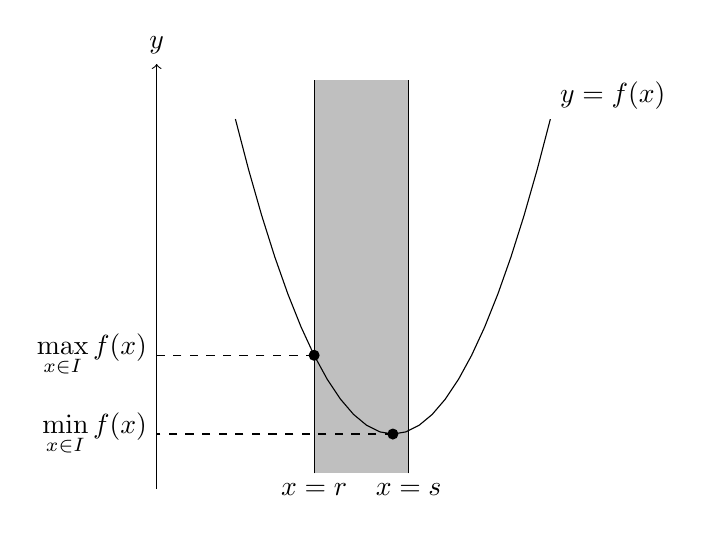
\begin{tikzpicture}
				\coordinate (r) at (-1,-0.5) node[below] at (r) {$x=r$};
				\coordinate (s) at ($(r)+(1.2,0)$) node[below] at (s) {$x=s$};
				\draw[->] (-3,-0.7) -- (-3,4.7) node[above] {$y$};
				\fill[lightgray] (r) |- ($(s)+(0,5)$) -- (s);
				\draw[domain=-2:2, name path=f] plot(\x,{pow(\x,2)}) node[above right] {$y=f(x)$};
				\fill (0,0) circle (2pt);
				\draw[name path=Lr] (r) -- ($(r)+(0,5)$);
				\draw[name path=Ls] (s) -- ($(s)+(0,5)$);
				\path[name intersections={
					of=Lr and f,
					by={intersection-r}
					}];
				\path[name intersections={
					of=Ls and f,
					by={intersection-s}
					}];
				\draw[dashed] (intersection-r) -- ($(intersection-r)-(r)+(-3,-0.5)$) node[left] {$\displaystyle\max_{x\in I}f(x)$};
				\fill (intersection-r) circle (2pt);
				\draw[dashed] (0,0) -- (-3,0) node[left] {$\displaystyle\min_{x\in I}f(x)$};
			\end{tikzpicture}
		\end{equation*}
		のような感じである.
		この場合,最大値は$f(r)\ (x=r)$,最小値は$q\ (x=p)$となる.
		
		ところで,今回の場合は$a>0$,つまり,$y=f(x)$のグラフが下に凸な場合を考えれば十分である.
		実際,$a<0$の場合は,$-f(x)$の最大と最小を入れ替えればよい.
		そこで,以下では$a>0$だとしよう.
		
		まずは最小値について考える.
		
		そもそも,実数上で$f(x)$は$x=p$において最小値$q$を取るから,$p\in I$の場合,つまり$r\le p\le s$の場合は,最小値が$q\ (x=p)$だと分かる.
		\begin{equation*}	%図
			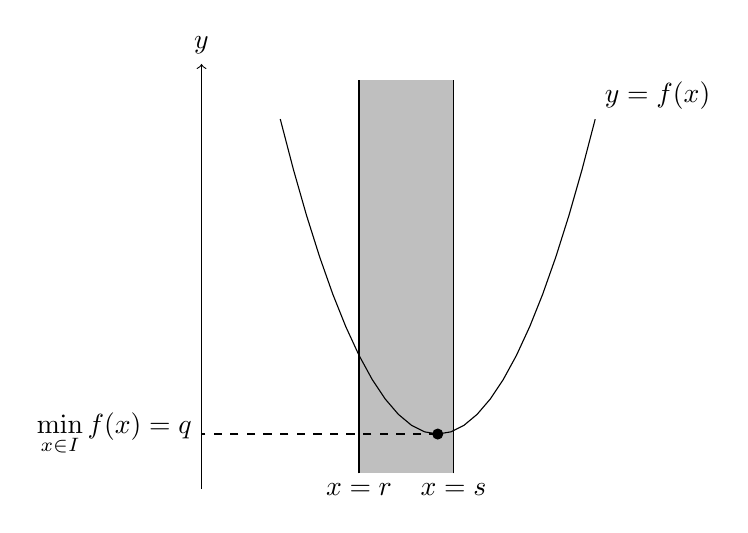
\begin{tikzpicture}[baseline=60]
				\coordinate (r) at (-1,-0.5) node[below] at (r) {$x=r$};
				\coordinate (s) at ($(r)+(1.2,0)$) node[below] at (s) {$x=s$};
				\draw[->] (-3,-0.7) -- (-3,4.7) node[above] {$y$};
				\fill[lightgray] (r) |- ($(s)+(0,5)$) -- (s);
				\draw[domain=-2:2, name path=f] plot(\x,{pow(\x,2)}) node[above right] {$y=f(x)$};
				\fill (0,0) circle (2pt);
				\draw[name path=Lr] (r) -- ($(r)+(0,5)$);
				\draw[name path=Ls] (s) -- ($(s)+(0,5)$);
				\path[name intersections={
					of=Lr and f,
					by={intersection-r}
				}];
				\path[name intersections={
					of=Ls and f,
					by={intersection-s}
				}];
				\draw[dashed] (0,0) -- (-3,0) node[left] {$\displaystyle\min_{x\in I}f(x)=q$};
			\end{tikzpicture}
		\end{equation*}
		
		後は,$p\notin I$の場合,つまり$p<r$または$s<p$である場合を考えればよい.
		この場合は,グラフの形から,$p<r$のときは$f(r)\ (x=r)$が最小値で,$s<p$のときは$f(s)\ (x=s)$が最小値だと分かる.
		\begin{align*}	%図
			&\text{$p<r$のとき}
			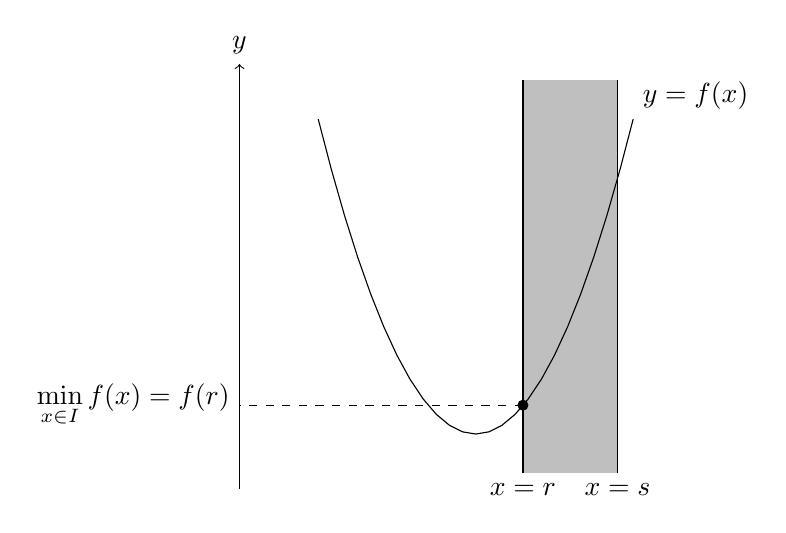
\begin{tikzpicture}[baseline=60]
				\coordinate (r) at (0.6,-0.5) node[below] at (r) {$x=r$};
				\coordinate (s) at ($(r)+(1.2,0)$) node[below] at (s) {$x=s$};
				\draw[->] (-3,-0.7) -- (-3,4.7) node[above] {$y$};
				\fill[lightgray] (r) |- ($(s)+(0,5)$) -- (s);
				\draw[domain=-2:2, name path=f] plot(\x,{pow(\x,2)}) node[above right] {$y=f(x)$};
				\draw[name path=Lr] (r) -- ($(r)+(0,5)$);
				\draw[name path=Ls] (s) -- ($(s)+(0,5)$);
				\path[name intersections={
					of=Lr and f,
					by={intersection-r}
				}];
				\path[name intersections={
					of=Ls and f,
					by={intersection-s}
				}];
				\draw[dashed] (intersection-r) -- ($(intersection-r)-(r)+(-3,-0.5)$) node[left] {$\displaystyle\min_{x\in I}f(x)=f(r)$};
				\fill (intersection-r) circle (2pt);
			\end{tikzpicture}\\
			&\text{$s<p$のとき}
			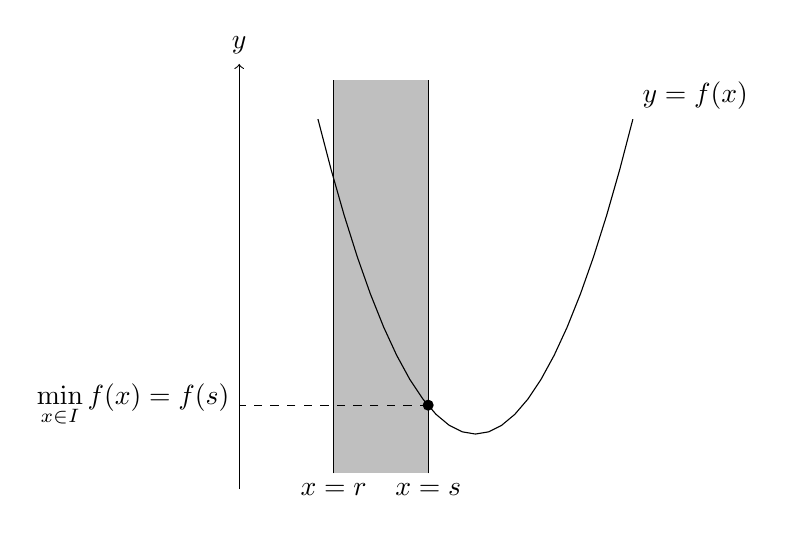
\begin{tikzpicture}[baseline=60]
				\coordinate (r) at (-1.8,-0.5) node[below] at (r) {$x=r$};
				\coordinate (s) at ($(r)+(1.2,0)$) node[below] at (s) {$x=s$};
				\draw[->] (-3,-0.7) -- (-3,4.7) node[above] {$y$};
				\fill[lightgray] (r) |- ($(s)+(0,5)$) -- (s);
				\draw[domain=-2:2, name path=f] plot(\x,{pow(\x,2)}) node[above right] {$y=f(x)$};
				\draw[name path=Lr] (r) -- ($(r)+(0,5)$);
				\draw[name path=Ls] (s) -- ($(s)+(0,5)$);
				\path[name intersections={
					of=Lr and f,
					by={intersection-r}
				}];
				\path[name intersections={
					of=Ls and f,
					by={intersection-s}
				}];
				\draw[dashed] (intersection-s) -- ($(intersection-s)-(s)+(-3,-0.5)$) node[left] {$\displaystyle\min_{x\in I}f(x)=f(s)$};
				\fill (intersection-s) circle (2pt);
			\end{tikzpicture}
		\end{align*}
		
		続いて,最大値について考える.
		$y=f(x)$のグラフは$x=p$に関して対称だから,$f(r)=f(s)$となる場合がある.
		これは,数直線上で$p$が$r$と$s$の中点である場合,つまり$p=\dfrac{r+s}{2}$である場合に対応する.
		このことは,グラフの対称性からも明らかだが,条件$f(r)=f(s)$から直接求めることもできる.
		実際,$f(r)=f(s)$なら
		\begin{align*}
			f(r)-f(s)=(r-s)(r+s-2p)=0
		\end{align*}
		であり,今は$r\ne s$としているので,$p=\dfrac{r+s}{2}$を得る.
		このとき,最大値は$f(r)\ (x=r,s)$である.
		\begin{equation*}
			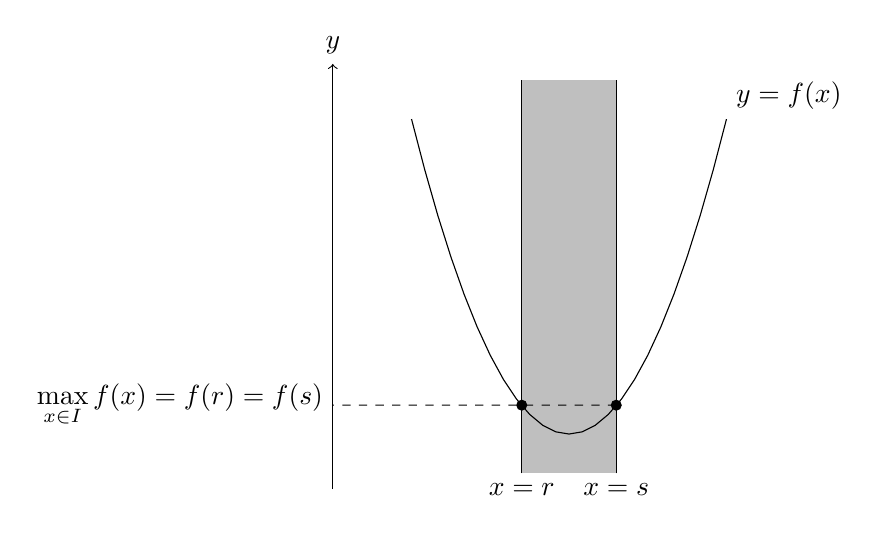
\begin{tikzpicture}
				\coordinate (r) at (-0.6,-0.5) node[below] at (r) {$x=r$};
				\coordinate (s) at ($(r)+(1.2,0)$) node[below] at (s) {$x=s$};
				\draw[->] (-3,-0.7) -- (-3,4.7) node[above] {$y$};
				\fill[lightgray] (r) |- ($(s)+(0,5)$) -- (s);
				\draw[domain=-2:2, name path=f] plot(\x,{pow(\x,2)}) node[above right] {$y=f(x)$};
				\draw[name path=Lr] (r) -- ($(r)+(0,5)$);
				\draw[name path=Ls] (s) -- ($(s)+(0,5)$);
				\path[name intersections={
					of=Lr and f,
					by={intersection-r}
				}];
				\path[name intersections={
					of=Ls and f,
					by={intersection-s}
				}];
				\draw[dashed] (intersection-s) -- ($(intersection-r)-(r)+(-3,-0.5)$) node[left] {$\displaystyle\max_{x\in I}f(x)=f(r)=f(s)$};
				\fill (intersection-r) circle (2pt);
				\fill (intersection-s) circle (2pt);
			\end{tikzpicture}
		\end{equation*}
		
		後は,$p\ne \dfrac{r+s}{2}$の場合を考えればよい.
		これは,$p\notin I$である場合の最小値を求めたときと同様に,グラフの形から,$p<\dfrac{r+s}{2}$のときは$f(s)\ (x=s)$が最大値で,$\dfrac{r+s}{2}<p$のときは$f(r)\ (x=r)$が最大値だと分かる.
		\begin{align*}	%図
			&\text{$p<\dfrac{r+s}{2}$のとき}
			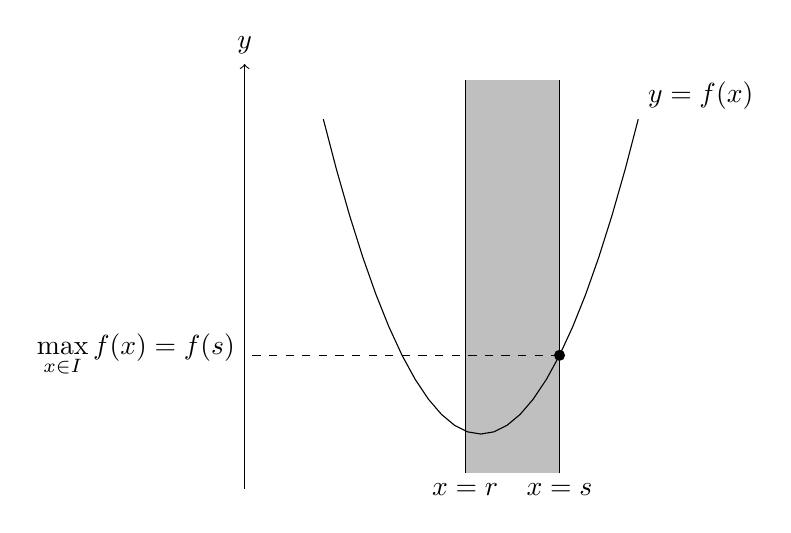
\begin{tikzpicture}[baseline=60]
				\coordinate (r) at (-0.2,-0.5) node[below] at (r) {$x=r$};
				\coordinate (s) at ($(r)+(1.2,0)$) node[below] at (s) {$x=s$};
				\draw[->] (-3,-0.7) -- (-3,4.7) node[above] {$y$};
				\fill[lightgray] (r) |- ($(s)+(0,5)$) -- (s);
				\draw[domain=-2:2, name path=f] plot(\x,{pow(\x,2)}) node[above right] {$y=f(x)$};
				\draw[name path=Lr] (r) -- ($(r)+(0,5)$);
				\draw[name path=Ls] (s) -- ($(s)+(0,5)$);
				\path[name intersections={
					of=Lr and f,
					by={intersection-r}
				}];
				\path[name intersections={
					of=Ls and f,
					by={intersection-s}
				}];
				\draw[dashed] (intersection-s) -- ($(intersection-s)-(s)+(-3,-0.5)$) node[left] {$\displaystyle\max_{x\in I}f(x)=f(s)$};
				\fill (intersection-s) circle (2pt);
			\end{tikzpicture}\\
			&\text{$\dfrac{r+s}{2}<p$のとき}
			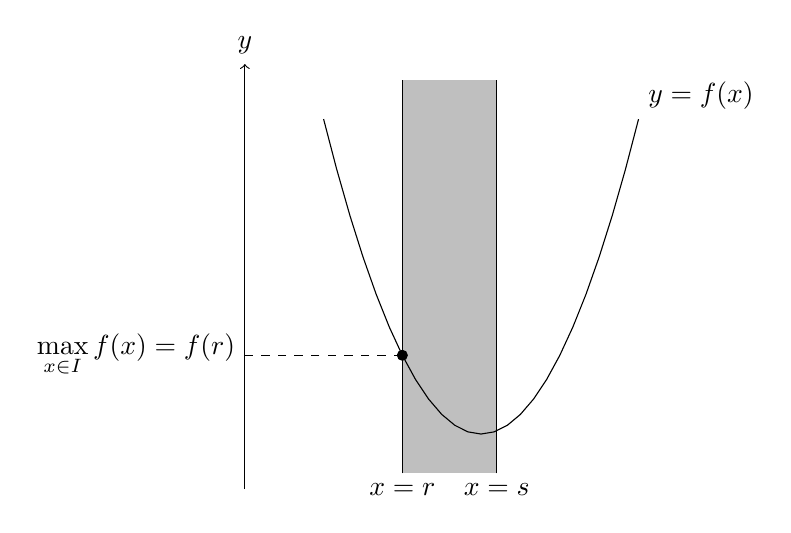
\begin{tikzpicture}[baseline=60]
				\coordinate (r) at (-1,-0.5) node[below] at (r) {$x=r$};
				\coordinate (s) at ($(r)+(1.2,0)$) node[below] at (s) {$x=s$};
				\draw[->] (-3,-0.7) -- (-3,4.7) node[above] {$y$};
				\fill[lightgray] (r) |- ($(s)+(0,5)$) -- (s);
				\draw[domain=-2:2, name path=f] plot(\x,{pow(\x,2)}) node[above right] {$y=f(x)$};
				\draw[name path=Lr] (r) -- ($(r)+(0,5)$);
				\draw[name path=Ls] (s) -- ($(s)+(0,5)$);
				\path[name intersections={
					of=Lr and f,
					by={intersection-r}
				}];
				\path[name intersections={
					of=Ls and f,
					by={intersection-s}
				}];
				\draw[dashed] (intersection-r) -- ($(intersection-r)-(r)+(-3,-0.5)$) node[left] {$\displaystyle\max_{x\in I}f(x)=f(r)$};
				\fill (intersection-r) circle (2pt);
			\end{tikzpicture}
		\end{align*}
		
		以上のことをまとめれば,下に凸な2次関数$f(x)=a(x-p)^2+q$の区間$[r,s]$における最大値,最小値について,
		\begin{alignat*}{2}
			&\text{$p<r$のとき\quad}
			&&\begin{cases}
				\text{最大値$f(s)$}	&(x=s),	\\
				\text{最小値$f(r)$}	&(x=r),
			\end{cases}\\
			&\text{$r\le p<\dfrac{r+s}{2}$のとき\quad}
			&&\begin{cases}
				\text{最大値$f(s)$}	&(x=s),	\\
				\text{最小値$q$}	&(x=p),
			\end{cases}\\
			&\text{$p=\dfrac{r+s}{2}$のとき\quad}
			&&\begin{cases}
				\text{最大値$f(s)=f(r)$}	&(x=r,s),	\\
				\text{最小値$q$}	&(x=p),
			\end{cases}\\
			&\text{$\dfrac{r+s}{2}<p\le s$のとき\quad}
			&&\begin{cases}
				\text{最大値$f(r)$}	&(x=r),	\\
				\text{最小値$q$}	&(x=p),
			\end{cases}\\
			&\text{$s<p$のとき\quad}
			&&\begin{cases}
				\text{最大値$f(r)$}	&(x=r),	\\
				\text{最小値$f(s)$}	&(x=s)
			\end{cases}\\
		\end{alignat*}
		が成り立つ.
		
		また,今回は$I$が有界な場合を考えたが,$I$が有界でない場合,例えば$I=(-\infty, s]$であるような場合についても,適切に解釈すれば,上にまとめたことが成り立つ.
		
		ここまで,最大値や最小値について考えたが,重要なのは区間と頂点の$x$座標の位置関係だと分かるだろう.
		つまり,各パラメータがどれだけ複雑になっても,関数の値ではなく,区間と頂点の位置関係にのみ注目すれば,問題は解けるはずである.
		
		ところで,上にまとめたものは,読者に暗記を促すものでは決してない.
		むしろ,整理するまでに述べた考え方をよく理解してほしい.
		
\end{document}
